\documentclass{standalone}
\usepackage{tikz}
\usetikzlibrary{patterns, positioning}
\usepackage[sfdefault]{ClearSans} %% option 'sfdefault' activates Clear Sans as the default text font
\usepackage[T1]{fontenc}

\begin{document}
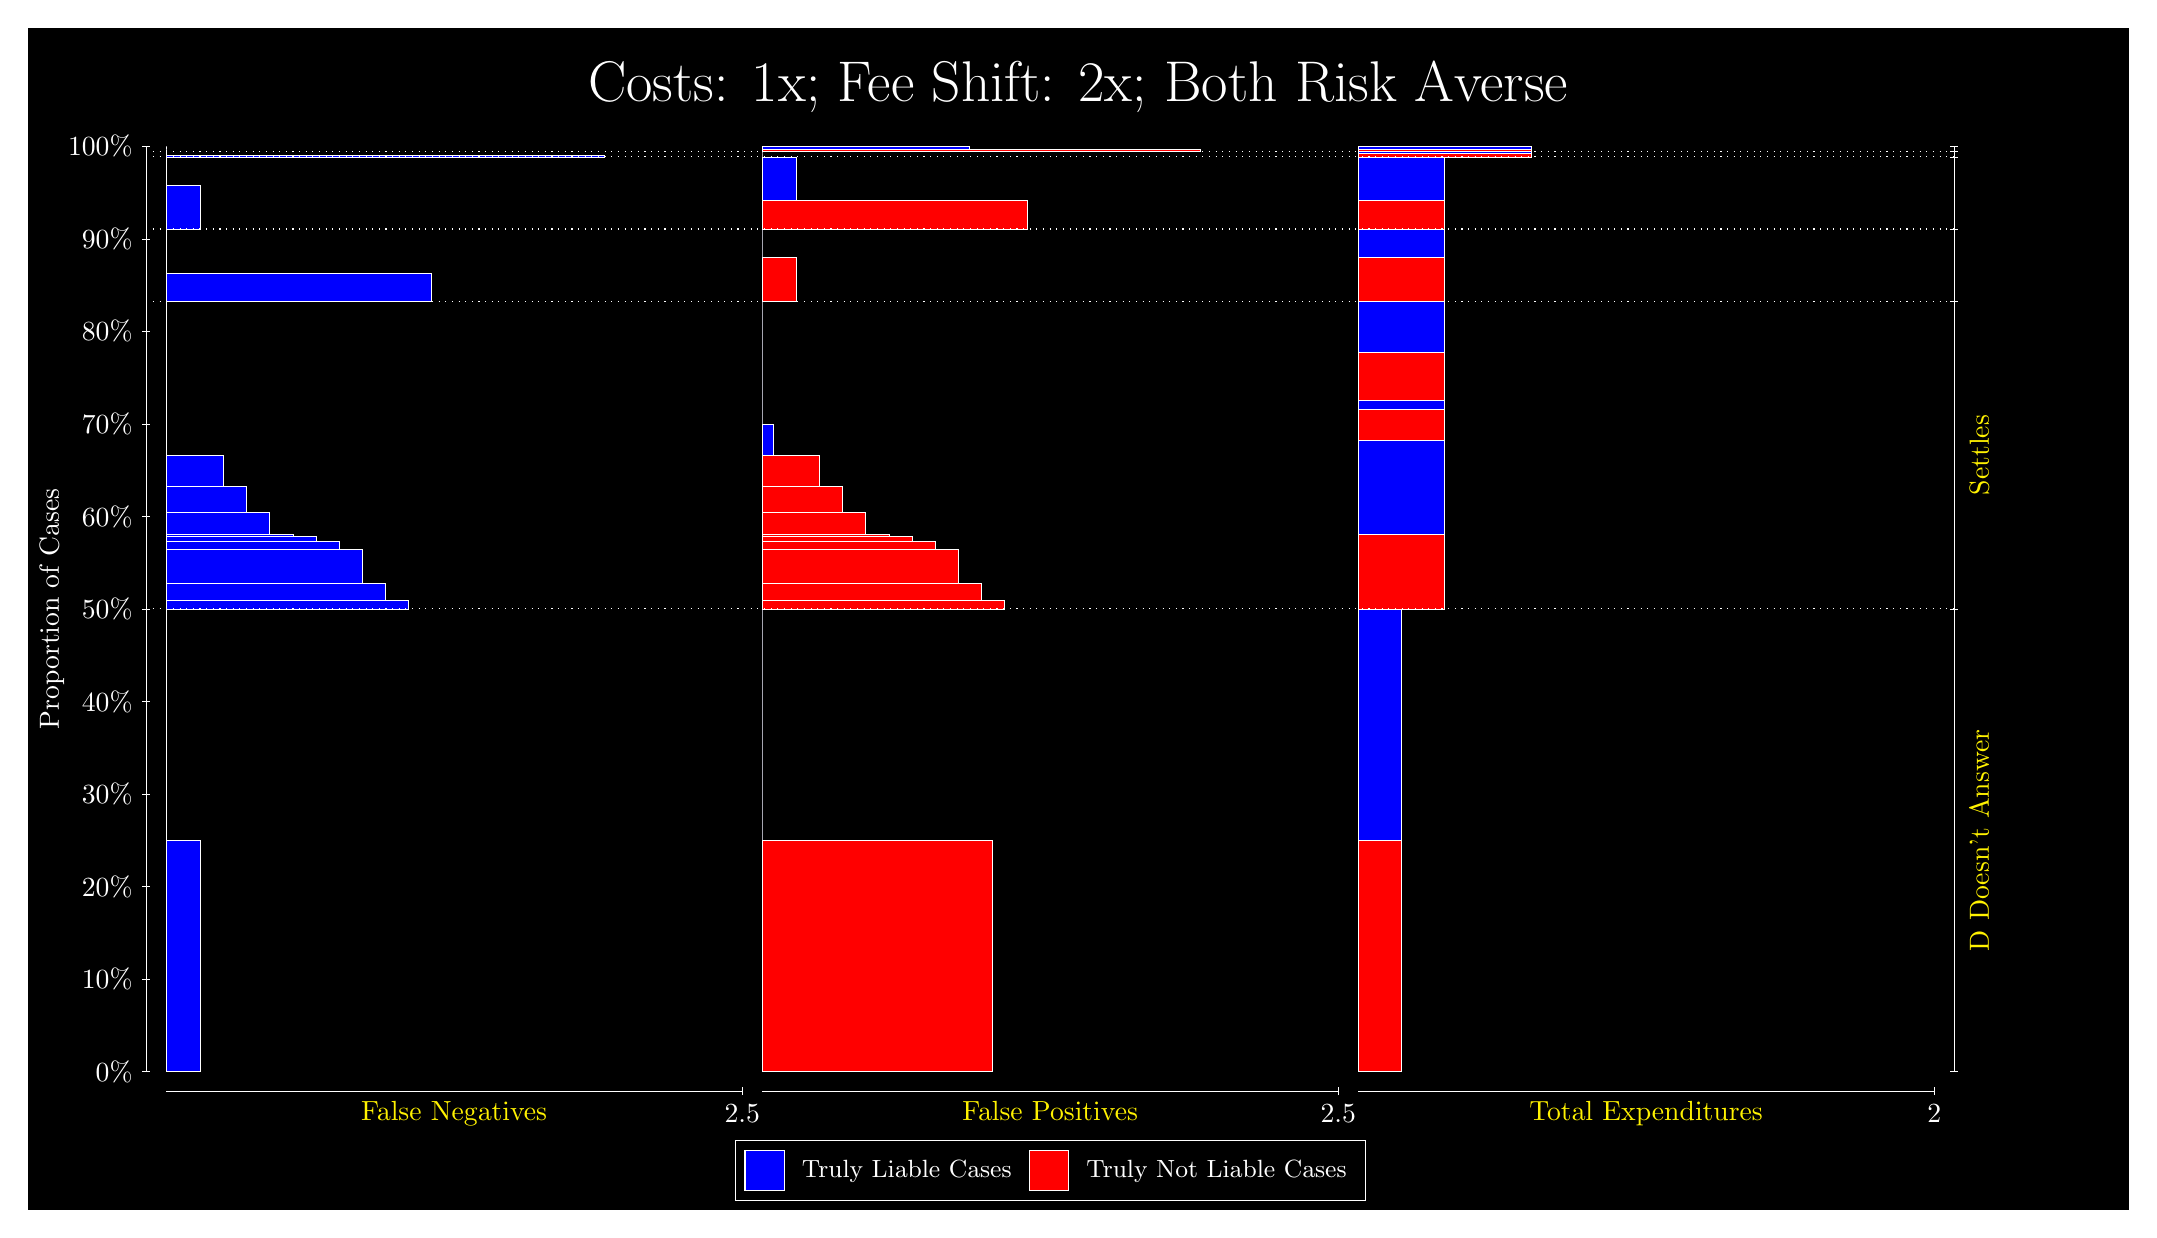
\begin{tikzpicture}
\draw[fill=black] (0,0) rectangle (26.667,15);
\draw[text=white] (0,13.5) rectangle (26.667,15) node[midway] {\huge Costs: 1x; Fee Shift: 2x; Both Risk Averse};
\draw[white, very thin] (1.5,1.75) -- (1.5,13.5);
\node[rotate=90, text=white, anchor=center] at (0.3, 7.625) {Proportion of Cases};
\draw[white, very thin] (1.45,1.75) -- (1.55,1.75);
\node[text=white, anchor=east] at (1.45, 1.75) {0\%};
\draw[white, very thin] (1.45,2.925) -- (1.55,2.925);
\node[text=white, anchor=east] at (1.45, 2.925) {10\%};
\draw[white, very thin] (1.45,4.1) -- (1.55,4.1);
\node[text=white, anchor=east] at (1.45, 4.1) {20\%};
\draw[white, very thin] (1.45,5.275) -- (1.55,5.275);
\node[text=white, anchor=east] at (1.45, 5.275) {30\%};
\draw[white, very thin] (1.45,6.45) -- (1.55,6.45);
\node[text=white, anchor=east] at (1.45, 6.45) {40\%};
\draw[white, very thin] (1.45,7.625) -- (1.55,7.625);
\node[text=white, anchor=east] at (1.45, 7.625) {50\%};
\draw[white, very thin] (1.45,8.8) -- (1.55,8.8);
\node[text=white, anchor=east] at (1.45, 8.8) {60\%};
\draw[white, very thin] (1.45,9.975) -- (1.55,9.975);
\node[text=white, anchor=east] at (1.45, 9.975) {70\%};
\draw[white, very thin] (1.45,11.15) -- (1.55,11.15);
\node[text=white, anchor=east] at (1.45, 11.15) {80\%};
\draw[white, very thin] (1.45,12.325) -- (1.55,12.325);
\node[text=white, anchor=east] at (1.45, 12.325) {90\%};
\draw[white, very thin] (1.45,13.5) -- (1.55,13.5);
\node[text=white, anchor=east] at (1.45, 13.5) {100\%};

\draw[white, very thin] (24.457,1.75) -- (24.457,13.5);
\draw[white, very thin] (24.407,1.75) -- (24.507,1.75);
\node[anchor=west] at (24.407, 1.75) {};
\draw[white, very thin] (24.407,7.625) -- (24.507,7.625);
\node[anchor=west] at (24.407, 7.625) {};
\draw[white, very thin] (24.407,11.532) -- (24.507,11.532);
\node[anchor=west] at (24.407, 11.532) {};
\draw[white, very thin] (24.407,12.45) -- (24.507,12.45);
\node[anchor=west] at (24.407, 12.45) {};
\draw[white, very thin] (24.407,13.367) -- (24.507,13.367);
\node[anchor=west] at (24.407, 13.367) {};
\draw[white, very thin] (24.407,13.433) -- (24.507,13.433);
\node[anchor=west] at (24.407, 13.433) {};
\draw[white, very thin] (24.407,13.5) -- (24.507,13.5);
\node[anchor=west] at (24.407, 13.5) {};

\draw[white, very thin, fill=blue] (1.75,1.75) rectangle (2.1891,4.6875);
\draw[white, very thin, fill=red] (1.75,4.6875) rectangle (1.75,7.625);
\draw[white, very thin, fill=blue] (1.75,7.625) rectangle (4.8239,7.7328);
\draw[white, very thin, fill=blue] (1.75,7.7328) rectangle (4.5312,7.951);
\draw[white, very thin, fill=blue] (1.75,7.951) rectangle (4.2384,8.3865);
\draw[white, very thin, fill=blue] (1.75,8.3865) rectangle (3.9457,8.4877);
\draw[white, very thin, fill=blue] (1.75,8.4877) rectangle (3.6529,8.5444);
\draw[white, very thin, fill=blue] (1.75,8.5444) rectangle (3.3602,8.578);
\draw[white, very thin, fill=blue] (1.75,8.578) rectangle (3.0674,8.8565);
\draw[white, very thin, fill=blue] (1.75,8.8565) rectangle (2.7746,9.1854);
\draw[white, very thin, fill=blue] (1.75,9.1854) rectangle (2.4819,9.5787);
\draw[white, very thin, fill=red] (1.75,9.5787) rectangle (1.75,11.532);
\draw[white, very thin, fill=blue] (1.75,11.532) rectangle (5.1167,11.893);
\draw[white, very thin, fill=red] (1.75,11.893) rectangle (1.75,12.45);
\draw[white, very thin, fill=blue] (1.75,12.45) rectangle (2.1891,13.006);
\draw[white, very thin, fill=red] (1.75,13.006) rectangle (1.75,13.367);
\draw[white, very thin, fill=blue] (1.75,13.367) rectangle (7.3123,13.392);
\draw[white, very thin, fill=red] (1.75,13.392) rectangle (1.75,13.433);
\draw[white, very thin, fill=red] (1.75,13.433) rectangle (1.75,13.458);
\draw[white, very thin, fill=blue] (1.75,13.458) rectangle (1.75,13.5);
\draw[white, very thin, fill=red] (9.3189,1.75) rectangle (12.246,4.6875);
\draw[white, very thin, fill=blue] (9.3189,4.6875) rectangle (9.3189,7.625);
\draw[white, very thin, fill=red] (9.3189,7.625) rectangle (12.393,7.7328);
\draw[white, very thin, fill=red] (9.3189,7.7328) rectangle (12.1,7.951);
\draw[white, very thin, fill=red] (9.3189,7.951) rectangle (11.807,8.3865);
\draw[white, very thin, fill=red] (9.3189,8.3865) rectangle (11.515,8.4876);
\draw[white, very thin, fill=red] (9.3189,8.4876) rectangle (11.222,8.5444);
\draw[white, very thin, fill=red] (9.3189,8.5444) rectangle (10.929,8.578);
\draw[white, very thin, fill=red] (9.3189,8.578) rectangle (10.636,8.8564);
\draw[white, very thin, fill=red] (9.3189,8.8564) rectangle (10.344,9.1853);
\draw[white, very thin, fill=red] (9.3189,9.1853) rectangle (10.051,9.5786);
\draw[white, very thin, fill=blue] (9.3189,9.5786) rectangle (9.4652,9.9719);
\draw[white, very thin, fill=blue] (9.3189,9.9719) rectangle (9.3189,11.532);
\draw[white, very thin, fill=red] (9.3189,11.532) rectangle (9.758,12.089);
\draw[white, very thin, fill=blue] (9.3189,12.089) rectangle (9.3189,12.45);
\draw[white, very thin, fill=red] (9.3189,12.45) rectangle (12.686,12.81);
\draw[white, very thin, fill=blue] (9.3189,12.81) rectangle (9.758,13.367);
\draw[white, very thin, fill=red] (9.3189,13.367) rectangle (9.3189,13.408);
\draw[white, very thin, fill=blue] (9.3189,13.408) rectangle (9.3189,13.433);
\draw[white, very thin, fill=red] (9.3189,13.433) rectangle (14.881,13.458);
\draw[white, very thin, fill=blue] (9.3189,13.458) rectangle (11.954,13.5);
\draw[white, very thin, fill=red] (16.888,1.75) rectangle (17.437,4.6875);
\draw[white, very thin, fill=blue] (16.888,4.6875) rectangle (17.437,7.625);
\draw[white, very thin, fill=red] (16.888,7.625) rectangle (17.986,8.578);
\draw[white, very thin, fill=blue] (16.888,8.578) rectangle (17.986,9.7702);
\draw[white, very thin, fill=red] (16.888,9.7702) rectangle (17.986,10.163);
\draw[white, very thin, fill=blue] (16.888,10.163) rectangle (17.986,10.271);
\draw[white, very thin, fill=red] (16.888,10.271) rectangle (17.986,10.879);
\draw[white, very thin, fill=blue] (16.888,10.879) rectangle (17.986,11.532);
\draw[white, very thin, fill=red] (16.888,11.532) rectangle (17.986,12.089);
\draw[white, very thin, fill=blue] (16.888,12.089) rectangle (17.986,12.45);
\draw[white, very thin, fill=red] (16.888,12.45) rectangle (17.986,12.81);
\draw[white, very thin, fill=blue] (16.888,12.81) rectangle (17.986,13.367);
\draw[white, very thin, fill=red] (16.888,13.367) rectangle (19.083,13.408);
\draw[white, very thin, fill=blue] (16.888,13.408) rectangle (19.083,13.433);
\draw[white, very thin, fill=red] (16.888,13.433) rectangle (19.083,13.458);
\draw[white, very thin, fill=blue] (16.888,13.458) rectangle (19.083,13.5);
\draw[white, dotted] (1.5,7.625) -- (24.457,7.625);
\draw[white, dotted] (1.5,11.532) -- (24.457,11.532);
\draw[white, dotted] (1.5,12.45) -- (24.457,12.45);
\draw[white, dotted] (1.5,13.367) -- (24.457,13.367);
\draw[white, dotted] (1.5,13.433) -- (24.457,13.433);
\draw[white, very thin] (1.75,1.5) -- (9.0689,1.5);
\node[text=yellow, anchor=north] at (5.4094, 1.5) {False Negatives};
\draw[white, very thin] (9.0689,1.45) -- (9.0689,1.55);
\node[text=white, anchor=north] at (9.0689, 1.45) {2.5};

\draw[white, very thin] (9.3189,1.5) -- (16.638,1.5);
\node[text=yellow, anchor=north] at (12.978, 1.5) {False Positives};
\draw[white, very thin] (16.638,1.45) -- (16.638,1.55);
\node[text=white, anchor=north] at (16.638, 1.45) {2.5};

\draw[white, very thin] (16.888,1.5) -- (24.207,1.5);
\node[text=yellow, anchor=north] at (20.547, 1.5) {Total Expenditures};
\draw[white, very thin] (24.207,1.45) -- (24.207,1.55);
\node[text=white, anchor=north] at (24.207, 1.45) {2};

\node[text=yellow, centered, rotate=90] at (24.777, 4.6875) {D Doesn't Answer};
\node[text=yellow, centered, rotate=90] at (24.777, 9.5786) {Settles};





\draw (12.978300999999998,1.5) node[draw=none] (baseCoordinate) {};
\begin{scope}[align=center]
        \matrix[scale=0.5, draw=white, below=0.5cm of baseCoordinate, nodes={draw}, column sep=0.1cm]{
            \node[rectangle, draw, minimum width=0.5cm, minimum height=0.5cm, fill=blue] {}; &
            \node[draw=none, font=\small, text=white] (B) {Truly Liable Cases}; &
            \node[rectangle, draw, minimum width=0.5cm, minimum height=0.5cm, fill=red] {}; &
            \node[draw=none, font=\small, text=white] (B) {Truly Not Liable Cases}; \\
            };
\end{scope}

\end{tikzpicture}
\end{document}